\section{Aprendizaje supervisado}

\code{popularity} es numérica, por lo que se compararon regresores. Una referencia
\code{DummyRegressor} con estrategia mediana fija el MAE que deben superar. Ridge
ofrece una combinación lineal regularizada ante atributos correlacionados; el árbol
de regresión captura umbrales e interacciones, con riesgo de sobreajuste. Se probaron
\code{alpha} 0,1; 1; 10 y 100 para Ridge, y profundidades 5, 10 o 15 con hojas
mínimas de 20 o 100 para el árbol. La regla fue menor MAE de validación, luego RMSE
y menor complejidad. No se usó la prueba para elegir parámetros.

\begin{table}[htbp]
\centering\small
\begin{tabular}{llrrrl}
\toprule
Predictores & Modelo & MAE & RMSE & $R^2$ & Configuración \\
\midrule
Completo & Ridge & 11,786 & 16,430 & 0,360 & $\alpha=0,1$ \\
Completo & Árbol & 14,393 & 18,312 & 0,205 & prof. 15; hoja 20 \\
Sin géneros & Ridge & 16,581 & 20,162 & 0,036 & $\alpha=0,1$ \\
Sin géneros & Árbol & 15,627 & 19,830 & 0,067 & prof. 15; hoja 20 \\
\bottomrule
\end{tabular}
\caption{Configuraciones seleccionadas en validación aleatoria; la referencia tuvo MAE 17,208.}
\label{tab:validation}
\end{table}

Tras reajustar cada configuración con las 71.792 canciones de entrenamiento, Ridge
completo obtuvo el menor MAE de la prueba aleatoria, como muestra la
Tabla~\ref{tab:random-test}. MAE y RMSE se expresan en puntos de popularidad.
$R^2$ compara el error cuadrático con una predicción constante igual a la media
observada de la prueba.

\begin{table}[htbp]
\centering\small
\begin{tabular}{llrrrr}
\toprule
Predictores & Modelo & MAE & RMSE & $R^2$ & Mejora MAE \\
\midrule
Referencia & Mediana & 17,250 & 20,612 & $\approx 0$ & 0,000 \\
Completo & Ridge & 11,915 & 16,643 & 0,348 & 5,335 \\
Completo & Árbol & 14,508 & 18,460 & 0,198 & 2,742 \\
Sin géneros & Ridge & 16,671 & 20,223 & 0,037 & 0,580 \\
Sin géneros & Árbol & 15,693 & 19,834 & 0,074 & 1,557 \\
\bottomrule
\end{tabular}
\caption{Prueba aleatoria reservada, $n=17.948$. La mejora MAE se calcula frente a la referencia mediana de esta misma prueba.}
\label{tab:random-test}
\end{table}

\begin{figure}[htbp]
\centering
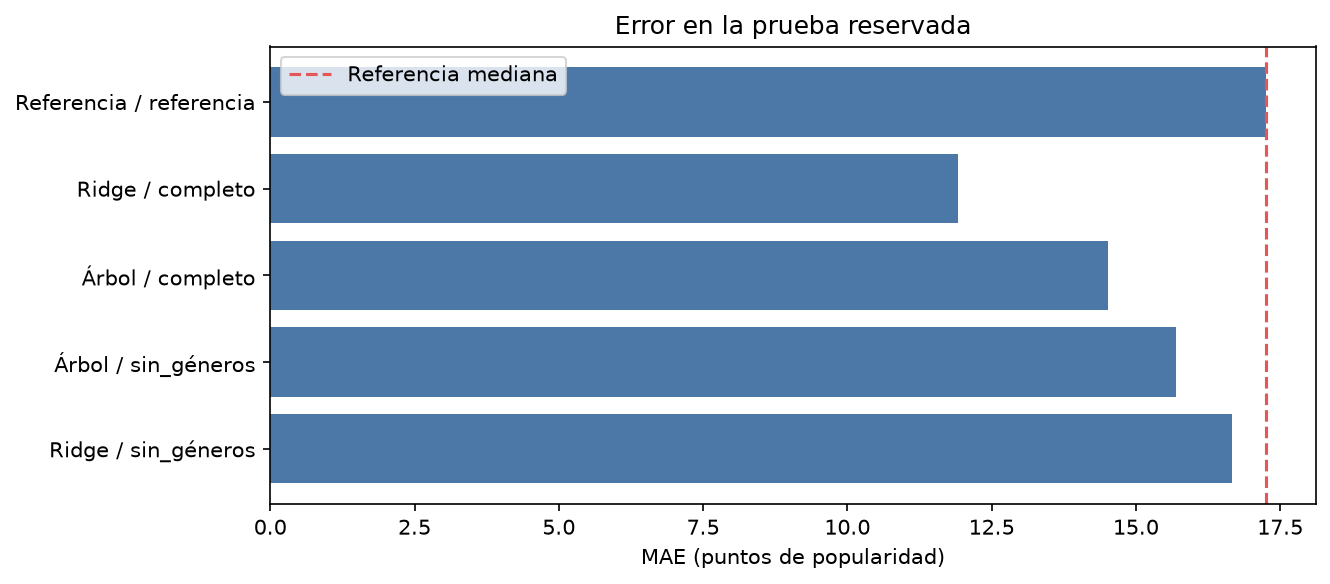
\includegraphics[width=0.91\linewidth]{04a_lucas_model_mae.png}
\caption{MAE de las configuraciones preseleccionadas en la prueba aleatoria. La línea vertical corresponde a la referencia mediana.}
\label{fig:model-mae}
\end{figure}

\subsection{Aporte de los géneros}

La ablación principal retira solo \code{track_genres} y conserva audio, estructura
musical y \code{explicit}. Bajo esa única diferencia, el MAE de Ridge aumenta
4,756 puntos (11,915 a 16,671) y el del árbol aumenta 1,186 (14,508 a 15,693).
En una comparación adicional \emph{solo de validación} se aislaron exactamente las
diez variables numéricas de audio, las etiquetas de género y ambas juntas; las
cuatro categóricas quedaron fuera para que los nombres de los conjuntos fueran
literales. Los mismos IDs y la misma regla de selección se usaron en cada variante.

\begin{table}[htbp]
\centering\small
\begin{tabular}{lrrrr}
\toprule
Variables & MAE Ridge & $R^2$ Ridge & MAE árbol & $R^2$ árbol \\
\midrule
Solo audio & 16,630 & 0,032 & 15,686 & 0,092 \\
Solo géneros & 11,849 & 0,355 & 14,472 & 0,204 \\
Audio y géneros & 11,800 & 0,358 & 14,391 & 0,204 \\
\bottomrule
\end{tabular}
\caption{Análisis adicional en los mismos 14.359 IDs de validación; no reabre la prueba aleatoria.}
\label{tab:feature-sets}
\end{table}

Con Ridge, añadir audio a solo géneros reduce el MAE de validación apenas 0,049
puntos. La señal de género sostiene casi todo el rendimiento de esa combinación
en esta muestra. No se puede cuantificar qué parte persistiría con una distribución
natural de géneros ni atribuir causalidad al género.
